\tracingstats=0
\iffalse\documentclass{article}\fi
\documentclass[12pt]{article}

\usepackage{sbc-template}
\usepackage{graphicx,url}
\usepackage{verbatim}

%sudo apt install texlive-lang-portuguese
\usepackage[portuguese]{babel}   
\usepackage[utf8]{inputenc} 
\usepackage{subfigure}
\usepackage{multirow}
\usepackage{graphicx}

\usepackage{algorithm}
\usepackage{algorithmicx}
\usepackage{algpseudocode}

%\usepackage[numbib,nottoc]{blindtext}
%\usepackage[numbib,nottoc]{tocbibind}

\graphicspath{ {./images/} } 

\sloppy

\title{Avaliação de superpixels para segmentação e detecção de contorno de imagens}

%Avaliar se superpixels podem ser utilizadas na segmentação de imagens sem diminuição do desempenho da segmentação, porém com custo inferior.

\author{Felipe Augusto Lima Reis\inst{1}}

\address{PUC Minas - Pontifícia Universidade Católica de Minas Gerais
  \email{falreis@sga.pucminas.br} }

\begin{document} 

\maketitle

\begin{abstract}
  Superpixels are structures that group similar pixels into sets that reflect aspects of the image. This paper evaluates the use of SLIC and EGB superpixels for segmentation. It's also evaluates the combination of both methods. Finally, this paper shows an hierarchical method implementation, using SLINK (single-linkage) clusterization, applied for the superpixels methods. For evaluation, this paper uses the Berkeley Segmentation Data Set (BSDS500). The results were compared to the dataset groundtruth, using precision and recall.
\end{abstract}
     
\begin{resumo} 
  Superpixels são estruturas que agrupam pixels semelhantes em conjuntos que refletem aspectos da imagem. Este artigo avalia a utilização de superpixels SLIC e EGB para segmentação. Avalia também os benefícios da combinação dos métodos para produção de segmentação. Por fim, o artigo mostra uma implementação de método hierárquico, utilizando clusterização SLINK (\textit{single-linkage}), para os métodos estudados nesse trabalho. Para avaliação dos resultados, foram utilizadas as imagens do conjunto de validação do Berkeley Segmentation Data Set (BSDS500). Os resultados foram com comparadas em relação ao \textit{groundtruth}, utilizando o método de precisão e revocação.
\end{resumo}


\section{Introdução} \label{sec:introducao}

A segmentação de imagens consiste em dividir uma imagem em um conjunto de regiões logicamente agrupadas, de modo a reunir áreas que contém informação relevante dentro dos grupos \cite{DOMINGUEZ}. Nessa tarefa, tomamos os \textit{pixels} como unidades básicas de processamento \cite{WANG201728}. O agrupamento de pixels em unidades maiores permite um tipo de segmentação chamado de \textit{oversegmentation} \cite{WANG201728}, ilustrado na Figura \ref{fig:superpixel}. O uso de superpixels possibilita o aumento da velocidade de processamento posterior, uma vez que a quantidade de pixels diminui consideravelmente em relação a imagem original.

\begin{figure}[ht]
\centering
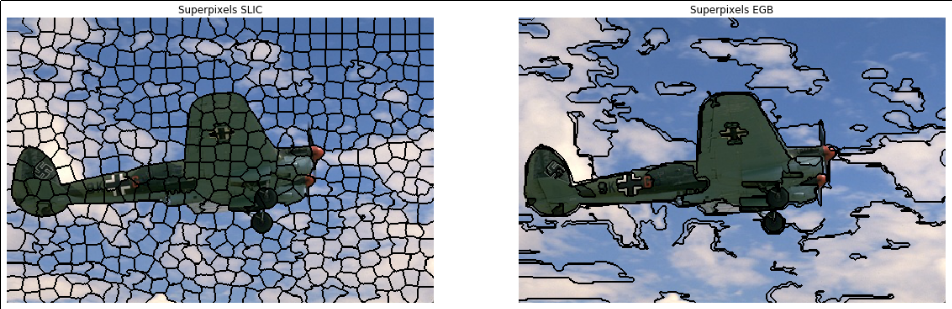
\includegraphics[width=1.\textwidth]{superpixels.png}
\caption{Imagens segmentadas utilizando superpixels SLICO e EGB}
\label{fig:superpixel}
\end{figure}

A utilização de superpixels possibilita a redução de itens a serem processados, entretanto pode causar perda de informação importante. No entanto, para alguns casos, a perda de qualidade pode se justificar em relação ao ganho de velocidade obtido utilizando esse tipo de operação. Essa relação consiste então em um \textit{trade-off} entre ambas as características, sendo viáveis em alguns cenários de processamento em tempo real ou para dispositivos com baixo desempenho.

Alguns métodos de geração de superpixels são utilizados para segmentação de imagens e detecção de bordas, como os métodos EGB \cite{FELZENSZWALB} e SLIC \cite{SLIC}. Esse trabalho investiga se a utilização de métodos segmentação e detecção de contornos baseados em superpixels.

O presente trabalho apresenta a seguinte estrutura: a Seção \ref{sec:ref_teorico} mostra o referencial teórico para construção do trabalho, a Seção  \ref{sec:mat_metodos}, exibe os materiais e métodos utilizados nos testes; a Seção \ref{sec:testes} mostra os resultados obtidos nos testes realizados e a discussões dos mesmos; a Seção \ref{sec:conclusao} contém a conclusão do artigo, com as considerações finais.

%%%%%%%%%%%%%%%%%%%%%%%%%%%%%%%%%%%%%%%%%%%%%%%%%%%%%%%
%%%%%%%%%%%%%%%%%%%%%%%%%%%%%%%%%%%%%%%%%%%%%%%%%%%%%%%
%%%%%%%%%%%%%%%%%%%%%%%%%%%%%%%%%%%%%%%%%%%%%%%%%%%%%%%


\section{Referencial Teórico} \label{sec:ref_teorico}

%%%%%%%%%%%%%%%%%%%%%%%%%%%%%%%%%%%%%%%%%%%%%%%%%%%%%%%
%%%%%%%%%%%%%%%%%%%%%%%%%%%%%%%%%%%%%%%%%%%%%%%%%%%%%%%

\subsection{Superpixels} \label{ssec:super}

Superpixels são estruturas que agrupam pixels semelhantes em conjuntos. O agrupamento possibilita a redução de complexidade das tarefas de processamento \cite{SLIC}, ao reduzir a quantidade de itens a serem processados. Os superpixels são utilizados na área de visão computacional para solução de vasto número de problemas, como detecção de contorno \cite{CONTOUR}, segmentação \cite{SEG_MERGE} e localização de objetos \cite{SEG_LOCALIZ}.

Superpixels, segundo \cite{FELZENSZWALB}, devem capturar importante grupos ou regiões, refletindo aspectos da imagem. Devem também ser executados em tempo próximo ao linear em relação a quantidade de pixels. Existem diversas abordagens para a geração de superpixels \cite{SLIC}. Dentre elas, podemos classificá-las, segundo o método de agrupamento em: 

\begin{itemize}
 \item \textit{Algoritmos baseados em grafos}: utilizam abordagem baseadas em grafos para correlação entre pixels e criação dos conjuntos. Dentre os algoritmos baseados em grafos podemos citar o \textit{Efficient Graph-Based Image Segmentation} (EGB) \cite{FELZENSZWALB};
 \item \textit{Algoritmos baseados em gradiente ascendente}: utilizam métodos de gradiente ascendente iterativamente até que os critérios de convergência correspondam a forma de um superpixel. Nesse conjunto, podemos  citar as abordagens \textit{watersheds} \cite{WATERSHEDS} \cite{SLIC}
 \item \textit{Algoritmos de clusterização iterativo}: utilizam métodos de clusterização, como o \textit{k-means}, para produção de superpixels. Um exemplo desse algoritmo é o SLIC (\textit{Simple Linear Iteravite Clustering}) \cite{SLIC}
\end{itemize}

%%%%%%%%%%%%%%%%%%%%%%%%%%%%%%%%%%%%%%%%%%%%%%%%%%%%%%%

\subsubsection{Superpixels SLIC} \label{sssec:slic}

O algoritmo SLIC utiliza um único parâmetro $k$, correspondente a quantidade aproximada de superpixels, gerados em formato regular \cite{SLIC}. A Figura \ref{fig:SLICO} ilustra o algoritmo SLIC para diferentes números de superpixels. A fim de produzir tamanhos semelhantes, o intervalo analisado é \mbox{$S=\sqrt{N/k}$}, onde $N$ é o número de pixels da imagem \cite{SLIC}. 

A definição do centro dos superpixels é feita utilizando sementes, que são movidas para locais de geração. Esses locais corresponem a posição mais baixa do gradiente em uma vizinhança de 3x3 \cite{SLIC}. Esse passo evita que superpixels sejam centrados nas bordas ou em um posição de ruído \cite{SLIC}. Cada pixel, então, é associado com o centro do cluster mais próximo, de modo que as regiões de busca se sobreponham \cite{SLIC}. A fim de aumentar o desempenho do algoritmo, a região de busca é limitada em 2 vezes o tamanho aproximado do superpixel $S$, gerando busca em uma área $2S \times 2S$ \cite{SLIC}. Em seguida, um passo de atualiza os centros dos clusters e computa o erro residual $E$ \cite{SLIC}. O algoritmo disponível no Algoritmo \ref{alg:SLIC}, resume as informações descrita nesse parágrafo.

\begin{algorithm}
    \caption{Segmentação por superpixels SLIC (\textit{Adaptado de } \cite{SLIC})}
    \label{alg:SLIC}
    \begin{algorithmic}[1]
        \State{\textit{ /* Inicialização */}}
        \State{Inicialize os centros dos clusters $C_k = [l_k, a_k, b_k, x_k, y_k]^T$ por amostragem de pixels em etapas de grade regulares $S$}
        \State{Mova os centros dos clusters para a posição de menor gradiente em uma vizinhança $3 \times 3$}
        \State{Faça label $l(i) = -1$ para cada pixel $i$}
        \State{Faça distância $d(i) = \infty $ para cada pixel $i$}
        \Repeat
            \For{cada cluster centrado em $C_k$}
                \For{cada pixel $i$ em uma região $2S \times 2S$ ao redor de $C_k$}
                \State{Compute a distância $D$ entre $C_k$ e $i$}
                \If{$D < d(i)$}
                    \State{faça $d(i) = D$}
                    \State{faça $l(i) = k$}
                \EndIf
                \EndFor
            \EndFor    
            \State{\textit{ /* Atualização */}}
            \State{Compute novos centros dos clusters}
            \State{Compute o erro residual $E$}
        \Until{$E \leq threshold$}
    \end{algorithmic}
\end{algorithm}


Para o algoritmo descrito na Figura \ref{alg:SLIC}, é necessário compreender o método para cálculo da medida de distância $D$ entre os conjuntos. Devido ao algoritmo trabalhar no \textit{colorspace} CIELAB, com o espaço-plano \textit{labxy}, a posição do pixel pode assumir um intervalo de valores. Com isso, o cálculo da distância não pode ser feito utilizando uma distância euclidiana, sendo necessária uma prévia normalização da proximidade espacial e de cor. Para isso é utilizado a fórmula $D=\sqrt{d_c^2+(d_s/S)^2 \cdot m^2}$, onde $D$ corresponde a distância em 5 dimensões do espaço labxy, $d_c$ e $d_s$ correspondem à proximidade de cores e proximidade espacial; e $m^2$ corresponde a distância máxima entre cores no cluster \cite{SLIC}. Para o cálculo da distância em imagens em escala cinza, é utilizada a distância Euclidiana \cite{SLIC}.

Uma etapa extra no processo de pós processamento é a união de \textit{pixels orfãos}. Esses pixels são adicionados ao cluster mais próximo usando o algoritmo de componentes conexos \cite{SLIC}.

Devido a limitação do espaço de pesquisa do algoritmo SLIC, a complexidade do algoritmo é $O(n)$, enquanto outros algoritmos que utilizam k-means para segmentação tem custo $O(k^N)$ \cite{SLIC}.

\begin{figure}[ht]
\centering
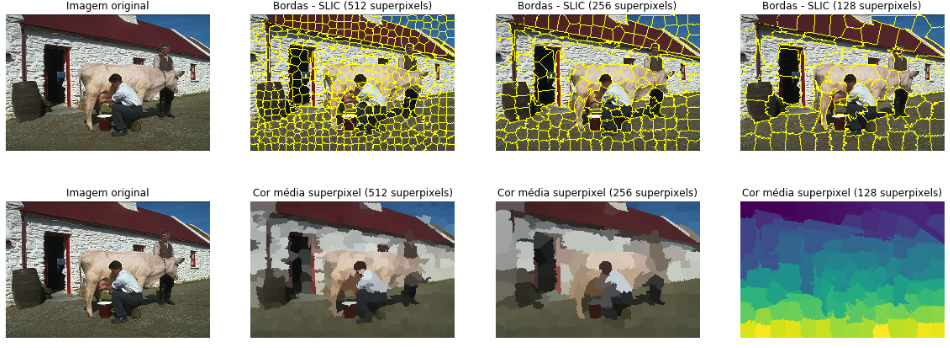
\includegraphics[width=1.\textwidth]{slic_segmentation_compare.png}
\caption{Fronteiras e coloração pelo valor médio dos superpixels SLIC/SLICO, para diferentes quantidades de superpixels}
\label{fig:SLICO}
\end{figure}

%%%%%%%%%%%%%%%%%%%%%%%%%%%%%%%%%%%%%%%%%%%%%%%%%%%%%%%

\subsubsection{Superpixels EGB} \label{sssec:egb}

Os superpixels EGB (\textit{Efficient Graph-Based Image Segmentation}) utilizam uma abordagem baseadas em grafos não direcionados. Nessa abordagem, cada \textit{pixel} corresponde a um nó do grafo e a ligação entre eles ocorre por meio de arestas, com pesos não negativos, correspondente a medida de dissimilaridade \cite{FELZENSZWALB}. 

Na abordagem baseada em grafos, a segmentação $S$ é uma partição dos vértices $V$ em componentes, no qual cada região $C \in S$ corresponde a um componente conectado em um grafo $G'=(V,E')$, onde $E' \subseteq E$, ou seja, a segmentação é induzida por um conjuntos de vértices em arestas $E$ \cite{FELZENSZWALB}.

No algoritmo foi definido um predicado $D$ para avaliação da evidência de bordas entre dois componentes de uma segmentação. O algoritmo avalia a dissimilaridade entre elementos de dois componentes e os compara com elementos vizinhos em um mesmo componente, de modo que o algoritmo possa se adaptar em relação as características dos dados \cite{FELZENSZWALB}. 

Para a comparação entre as regiões é utilizada uma função de corte (\textit{threshold}) $\tau$, a fim de medir o grau de diferença entre os componentes. Esse grau deve ser superior a diferença interna mínima, evidenciando uma borda \cite{FELZENSZWALB}. A função de corte, no algoritmo, é utilizada baseado no tamanho do componente $\tau=k/|C|$, onde $|C|$ corresponde ao tamanho do componente $C$ e $k$ corresponde a um parâmetro do algoritmo \cite{FELZENSZWALB}.

O algoritmo EGB, utilizando pesos inteiros e ordenação por contagem, pode ser executado com custo linear, com complexidade $O(nlogn)$, para qualquer método de ordenação \cite{FELZENSZWALB}. 

\begin{figure}[ht]
\centering
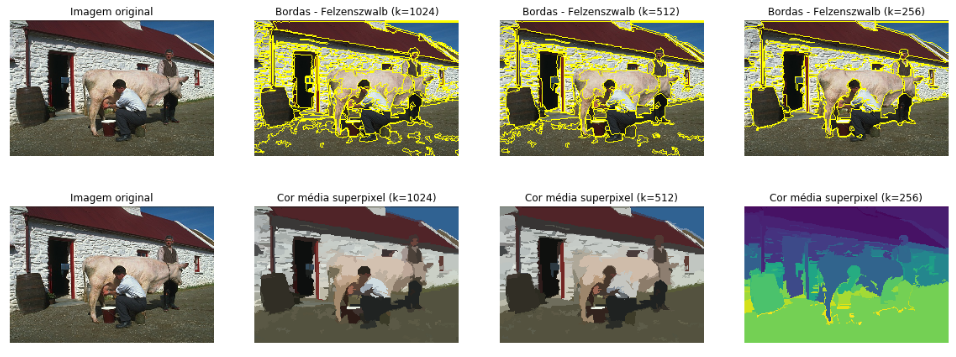
\includegraphics[width=1.\textwidth]{felz_segmentation_compare.png}
\caption{Fronteiras e coloração pelo valor médio dos superpixels EGB, para diferentes quantidades de superpixels}
\label{fig:EGB}
\end{figure}

%%%%%%%%%%%%%%%%%%%%%%%%%%%%%%%%%%%%%%%%%%%%%%%%%%%%%%%
%%%%%%%%%%%%%%%%%%%%%%%%%%%%%%%%%%%%%%%%%%%%%%%%%%%%%%%

\subsection{Clusters} \label{ssec:clusters}

% Análise de cluster é a tarefa de agrupar dados em grupos (\textit{clusters}) que tenham características em comum, sejam signinficativos e/ou úteis \cite{CLUSTER_HIER}. \textit{Clusters} hierárquicos correspondem a análise de \textit{clusters} a fim de buscar hierarquias entre eles. As estratégias para hierarquização de cluster se dividem em dois grupos \cite{ROKACH}:

\begin{itemize}
 \item Aglomerativo - abordagem \textit{"bottom up"}, em que a observação inicia-se no próprio \textit{cluster} e os pares de \textit{clusters} são unidos na medida em que se sobe na hierarquia. 
 \item Divisivo - abordagem \textit{"top down"} onde as observações iniciam-se em um \textit{cluster} e são realizadas recursivamente a medida em que se desce na hierarquia.
\end{itemize}

Os algoritmos originais de cluster possuem complexidade $O(n^3)$. Alguns algoritmos, entretanto, como o SLINK, ou \textit{single-linkage}, possuem complexidade $O(n^2)$ \cite{SLINK}. O SLINK utiliza a distância mínima como critério de ligação (\textit{linkage}) entre os \textit{clusters}. A fórmula $min\{d(a,b): a \in A, b \in B \}$, corresponde a distância mínima para dois pares de clusters A e B observados, onde $d$ é a métrica de distância escolhida \cite{WIKI_CLUSTER_HIERARCHY}.

A partir da aglomeração de clusters é possivel construir uma árvore hierarquica, onde os clusters são agrupados por sua similaridade. Um método de visualização dessas características é o dendrograma. 

%%%%%%%%%%%%%%%%%%%%%%%%%%%%%%%%%%%%%%%%%%%%%%%%%%%%%%%
%%%%%%%%%%%%%%%%%%%%%%%%%%%%%%%%%%%%%%%%%%%%%%%%%%%%%%%

\subsection{Detecção de Contornos e Segmentação de Imagens} \label{ssec:segmentacao}

Segmentação de imagens consiste em separar uma imagem em regiões, idealmente correspondente a objetos reais \cite{ZHANG2008}. Esse passo é utilizado no processamento de imagens, vídeos e aplicações de visão computacional. Também consiste em um importante passo na tentativa de explicar uma imagem por meio de algoritmos \cite{ZHANG2008}.

Extensiva pesquisa é realizada e muitas abordagens e algoritmos são utilizados, com bons resultados para um conjunto ou classes de imagens \cite{ZHANG2008}. A fim de facilitar a pesquisa, alguns trabalhos foram desenvolvidos para criação de um conjunto de imagens com suas respectivas segmentações manuais. A base BSDS500 (\textit{Berkeley Segmentation Data Set and Benchmarks 500}) provê uma base de imagens para pesquisa de segmentação e detecção de bordas. \cite{BSDS500}. Essa base de dados é uma extensão da base BSDS300, com 200 novas imagens para avaliação \cite{BSDS500}.

A fim de avaliar a efetividade das segmentações, tradicionalmente são utilizados métodos subjetivos, como a visualização humana, responsável por comparar a qualidade da segmentação ou métodos supervisionados, onde uma segmentação é comparada em relação a uma imagem manualmente segmentada \cite{ZHANG2008}. Projetos de detecção automática, como o SEISM (\textit{Supervised Evaluation of Image Segmentation Methods}) permitem a avaliação da segmentação, usando a recuperação de precisão para bordas e a recuperação de precisão para objetos e peças \cite{SEISM}.

%%%%%%%%%%%%%%%%%%%%%%%%%%%%%%%%%%%%%%%%%%%%%%%%%%%%%%%
%%%%%%%%%%%%%%%%%%%%%%%%%%%%%%%%%%%%%%%%%%%%%%%%%%%%%%%
%%%%%%%%%%%%%%%%%%%%%%%%%%%%%%%%%%%%%%%%%%%%%%%%%%%%%%%

\section{Materiais e Métodos} \label{sec:mat_metodos}

Para confecção do trabalho foram escolhidos os algoritmos de SLIC e EGB. Os algoritmos possuem características diferentes: o SLIC é capaz de produzir \textit{superpixels} em formas regulares, porém não é tão preciso ao separar os conjuntos por similaridade; por outro lado, o EGB, produz \textit{superpixels} irregulares, porém é mais aderente às diferenças de cores entre \textit{pixels}.

Nos testes realizados foi realizada hierarquização dos resultados obtidos após a geração de superpixels SLIC, EGB e também sobre a composição SLIC+EGB. A composição SLIC+EGB corresponde a aplicação do algoritmo SLIC, seguido pela recoloração utilizando o valor médio de cores do \textit{superpixel} e, por fim, a aplicação do método EGB. A partir dessa seção, o método SLIC+EGB passará a ser chamado SEGB, para facilitar a nomenclatura.

Os resultados das hierarquizações foram comparados aos melhores resultados de segmentação obtidos pela segmentação SLIC, EGB e SEGB sem hierarquização. O método de hierarquização está descrito na seção \ref{ssec:hierquia_segm}, enquanto o método de avaliação de resultados está descrito na seção \ref{ssec:aval_resultados}. Os resultados dos testes estão disponíveis na seção \ref{sec:testes}.

%%%%%%%%%%%%%%%%%%%%%%%%%%%%%%%%%%%%%%%%%%%%%%%%%%%%%%%
%%%%%%%%%%%%%%%%%%%%%%%%%%%%%%%%%%%%%%%%%%%%%%%%%%%%%%%

\subsection{Hierarquia de Segmentações} \label{ssec:hierquia_segm}

% %%%%%%%%%%%%%%%%%%%%%%%%%%%%%%%%%%%%%%%%%%%%%%%%%%%%%%%

A hierarquização das segmentações tem como objetivo possibilitar a utilização dos algoritmos para produzir segmentação em diferentes níveis de detalhamento: desde um nível mais aprofundado até um nível macro. Os diferentes níveis hierárquicos podem ser combinados em termos do contorno das hierárquias, permitindo a representação das hierarquias indexadas como bordas suaves, chamadas Mapas de Contorno Ultramétrico (UCM - \textit{Ultrametric Contour Map}) \cite{ULTRAMETRIC}.

Para construção das hierarquias foram gerados \textit{clusters} com as correlações entre os grupos de \textit{superpixels} adjcentes, após a segmentação inicial. Foi utilizado o algoritmo SLINK (\textit{single-linkage}) para agrupamento dos \textit{superpixels} próximos, gerando uma árvore com as correlações entre os \textit{superpixels}.

Para verificação da estrutura da árvore foi utilizado um dendrograma, como representado na Figura \ref{fig:DENDROGRAM}. O dendrograma é um tipo de árvore utilizado para ilustração de uma clusterização hierarquica \cite{WIKI_DENDROGRAM}. Frequentemente é utilizado nas áreas de biologia para indicar a mudanças evolucionárias entre ancestrais e descendentes, baseados em suas características \cite{DENDROGRAM}.

\begin{figure}[ht]
\centering
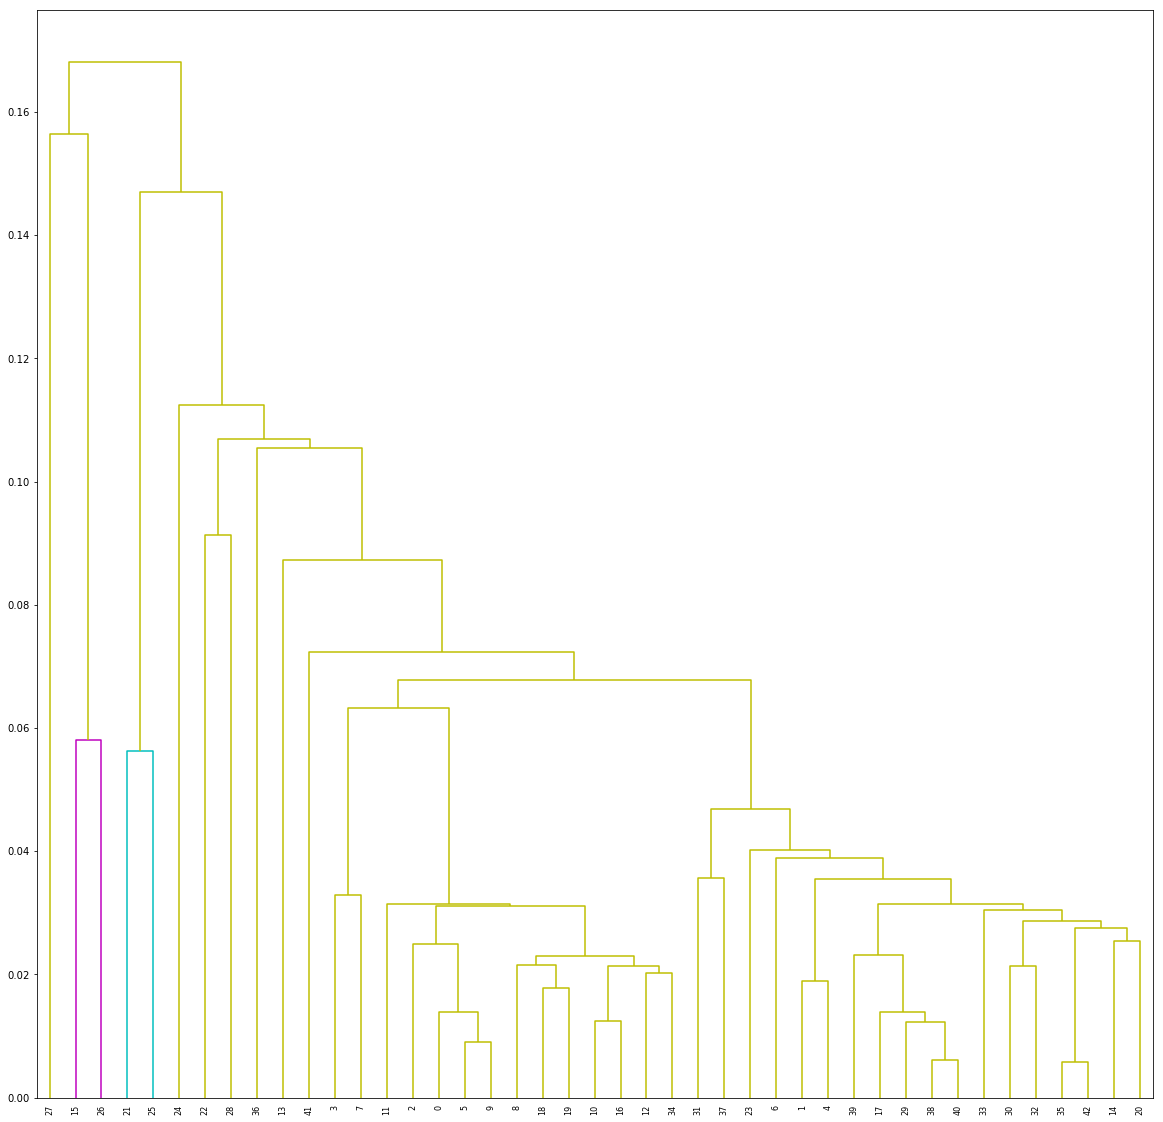
\includegraphics[width=1.\textwidth]{dendrogram.png}
\caption{Dendrograma dos superpixels de uma imagem}
\label{fig:DENDROGRAM}
\end{figure}

Em um árvore de estrutura semelhante à representada por um dendrograma é possível realizar cortes horizontais ou verticais na hierarquia, a fim de obter tipos de agrupamentos diferentes. No trabalho realizado somente foram realizados cortes horizontais, em diversos níveis. 

Devido às características da segmentação, quando comparados ao \textit{groundtruth}, não foram validados todos os níveis hierárquicos. A fim de reduzir o número de comparações, somente foram avaliados níveis hierárquicos intermediários que apresentaram melhores resultados em testes empíricos. Com isso, foi estabelecido um limite máximo e mínimo para os cortes na hierarquia, de modo que os cortes foram feitos dentro de um intervalo, evitando avalição de níveis com baixa probabilidade adequação ao \textit{groundtruth}.

%%%%%%%%%%%%%%%%%%%%%%%%%%%%%%%%%%%%%%%%%%%%%%%%%%%%%%%
%%%%%%%%%%%%%%%%%%%%%%%%%%%%%%%%%%%%%%%%%%%%%%%%%%%%%%%

\subsection{Análise Multiescala} \label{ssec:analise_multiescala}

Para que os níveis hierarquicos possam garantir a manutenção da informação, agrupando apenas características semelhantes, as hierarquias devem seguir os princípios de análise multiescala \cite{SILVIO_ZENILTON}. Esses princípios asseguram manutenção de duas características principais \cite{SILVIO_ZENILTON}:

\begin{itemize}
 \item Causalidade - um contorno presente em uma escala $k1$ deve estar presente em qualquer escala $k2 < k1$ \cite{SILVIO_ZENILTON};
 \item Localidade - a medida em que o número de regiões diminui, os contornos devem ser estáveis (não devem se mover). A união corresponde a manutenção das bordas dos grupos que se fundiram \cite{SILVIO_ZENILTON}.
\end{itemize}

O método de hierarquização descrito nesse trabalho manteve as características da análise multiescala. A Figura \ref{fig:hierarq_partit} mostra os possíveis cortes na hierarquia de uma segmentação SEGB, sem recoloração da imagem. Nesse modelo, a segmentação é capaz de unir pixels por similaridade.

É importante salientar que os métodos originais (SLIC e EGB), quando apenas variados os parâmetros de criação de superpixels não mantém as características de análise multiescala, conforme podemos ver nas Figuras \ref{fig:SLICO} e \ref{fig:EGB}; essas características somente são obtidas pelos processos hierárquicos aplicados aos métodos após a criação dos superpixels.

\begin{figure}[ht]
\centering
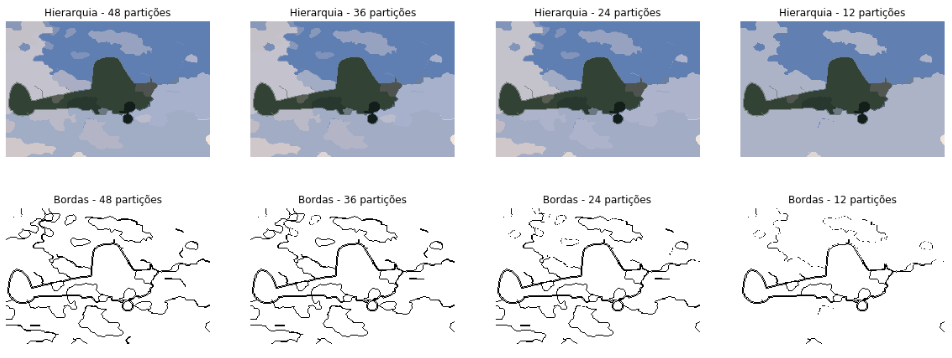
\includegraphics[width=1.\textwidth]{slic_hierarquia_particoes.png}
\caption{Hierarquia de partições utilizando superpixel SLIC+EGB.}
\label{fig:hierarq_partit}
\end{figure}


%%%%%%%%%%%%%%%%%%%%%%%%%%%%%%%%%%%%%%%%%%%%%%%%%%%%%%%
%%%%%%%%%%%%%%%%%%%%%%%%%%%%%%%%%%%%%%%%%%%%%%%%%%%%%%%

\subsection{Avaliação de Resultados} \label{ssec:aval_resultados}

Para avaliação das imagens, foi primeiramente utilizada a classificação visual, comparando a qualidade dos resultados. Em seguida utilizou-se um método de comparação de precisão e revocação, para detecção de contornos e bordas.

O método de precisão é um método de classificação binária, onde a precisão (\textit{prediction}) corresponde à ``fração de instâncias recuperadas que são relevantes'', enquanto revocação (\textit{recall}), corresponde ``a fração de instâncias relevantes que são recuperadas'' \cite{WIKI_PREC_RECALL}. Ambos os métodos são avaliados juntos para que possam identificar 4 tipos de dados possíveis:

\begin{itemize}
 \item Verdadeiros Positivos - correspondem aos valores que foram corretamente classificados como positivos;
 \item Falsos Negativos - correspondem aos valores que foram classificados incorretamente como negativos;
 \item Falsos Positivos - correspondem aos valores que foram classificados incorretamente como positivos;
 \item Verdadeiros Negativos - correspondem aos valores que foram classificados corretamente como negativos \cite{WIKI_PREC_RECALL};
\end{itemize}

A classificação descrita acima está ilustrada na Figura \ref{fig:PREC_RECALL}. 

\begin{figure}[ht]
\centering
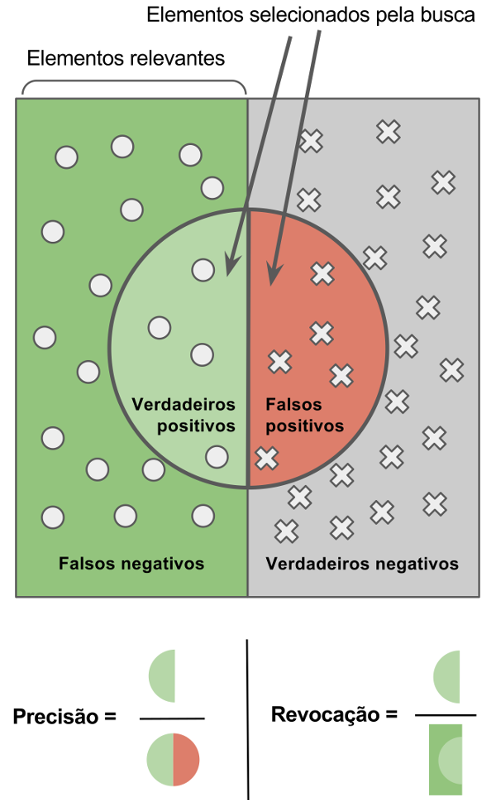
\includegraphics[width=0.4\textwidth]{precision_recall.png}
\caption{Precisão e revocação. Adaptado de \cite{WIKI_PREC_RECALL}}
\label{fig:PREC_RECALL}
\end{figure}

A classificação de precisão e revocação pode ser dada por uma média harmônica, chamada de \textit{F-measure} ou \textit{F-score} balanceada. Essa medida é dada pela fórmula \cite{WIKI_PREC_RECALL}:

\begin{equation}
 F=2 \cdot \frac{precis \cdot revoc}{precis + revoc}
\end{equation}

A medida é aproximadamente a média quando seus valores estão próximos, porém o valor é baixo quando as médias estão distantes, favorecendo métodos com baixo número de falsos positivos e verdadeiros negativos \cite{WIKI_PREC_RECALL}

%%%%%%%%%%%%%%%%%%%%%%%%%%%%%%%%%%%%%%%%%%%%%%%%%%%%%%%
%%%%%%%%%%%%%%%%%%%%%%%%%%%%%%%%%%%%%%%%%%%%%%%%%%%%%%%

\subsection{Código Fonte e Bibliotecas Utilizados} \label{ssec:cod_fonte}

Os códigos fontes gerados, realizando as segmentações, hierarquias, geração de mapas ultramétricos, avaliação dos resultados e os gráficos presentes nesse trabalhos estão disponíveis publicamente na página pessoal do autor no Github \footnote{https://github.com/falreis/image-segm}.

Os algoritmos SLIC e EGB utilizados para realização desse trabalho foram obtidos pela biblioteca Scikit-Image\footnote{http://scikit-image.org/docs/dev/api/skimage.segmentation.html}.
Os algoritmos de geração de cluster SLINK e representação de dendrogramas foram obtido na biblioteca Scipy.org\footnote{https://docs.scipy.org/doc/scipy-0.18.1/reference/generated/scipy.cluster.hierarchy.linkage.html}. 
O algoritmo de avaliação do resultado foi obtido no projeto Image-Segmentation, no Github\footnote{https://github.com/Htiango/Image-Segmentation/blob/master/main/eval\_boundary.py}. 

%Também foi utilizado o benchmarks de avaliação de performance das segmentações, disponíveis na base de dados BSDS500\footnote{https://www2.eecs.berkeley.edu/Research/Projects/CS/vision/grouping/resources.html}.


%%%%%%%%%%%%%%%%%%%%%%%%%%%%%%%%%%%%%%%%%%%%%%%%%%%%%%%
%%%%%%%%%%%%%%%%%%%%%%%%%%%%%%%%%%%%%%%%%%%%%%%%%%%%%%%
%%%%%%%%%%%%%%%%%%%%%%%%%%%%%%%%%%%%%%%%%%%%%%%%%%%%%%%


\section{Testes, Resultados e Discussões} \label{sec:testes}

Para avaliação do desempenho dos algoritmos foi executada a segmentação das imagens do conjunto de validação da base de dados  BSDB500 (\textit{Berkeley Segmentation Data Set}). O conjunto possui 100 imagens naturais com seus respectivos \textit{groundtruths} feito por anotações humanas \cite{BSDS500}. 

Os algoritmos foram aplicados a base de testes e comparados com os \textit{groundtruths} disponíveis na base de dados. A adequação do algoritmo em relação ao \textit{ground-truth} foi feita por meio do mecanismo de precisão e revocação, utilizando a medida \textit{F-measure}, conforme descrito na seção \ref{ssec:aval_resultados}.

A  fim de obter a melhor parametrização possível, foram executados diversos testes para cada algoritmo. Somente o algoritmo EGB não foi extensamente executado a fim de obter a melhor parametrização, uma vez que os valores obtidos pelos autores estão disponíveis no artigo \textit{Efficient Graph-Based Image Segmentation} \cite{FELZENSZWALB}. A parametrização dos algoritmos está detalhada na Tabela \ref{table:PARAMETROS}.

\begin{table}
  \begin{center}
  \begin{tabular}{| l | c | c | c |}
  \hline & \multicolumn{3}{ |c| }{Algoritmos} \\
  \hline %\multirow{4}{*}{Parâmetros} 
    & SLIC & EGB & SEGB \\ 
  \hline
    $k$ & 300 & - & 1408 \\
  \hline
    $scale$ & - & 300 & 1408 \\
  \hline
    $sigma$ & - & 0.8 & 0.8 \\ 
  \hline
    $min\_size$ & - & 30 & 30 \\
  \hline
  \end{tabular}
  \caption{Parametrização dos algoritmos.}
  \label{table:PARAMETROS}
  \end{center}
\end{table}

Os algoritmos hierárquicos foram executados e a melhor partição obtida para todo o conjunto de imagens (ODS - \textit{Optimal Data Set Scale}) \cite{CONT_EMPIRICAL} foi utilizada. Em seguida os valores foram comparados aos demais algoritmos utilizando com métrica a medida \textit{F-measure}. A eficiência média dos algoritmos está ilustrada na Figura \ref{fig:FMEASURE_AVG}.

\begin{comment}

\begin{figure}[ht]
 \subfigure[Valor médio]{\label{fig:FMEASURE_AVG}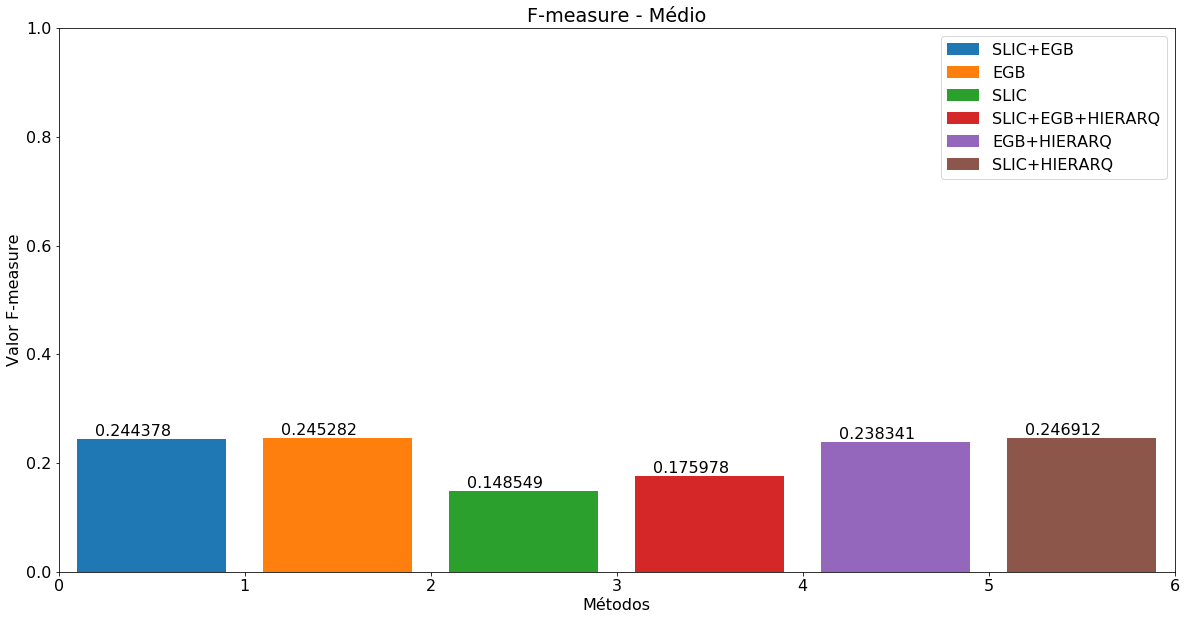
\includegraphics[width=0.5\linewidth]{fmeasure_avg.png}}
 \subfigure[Valor máximo]{\label{fig:FMEASURE_MAX}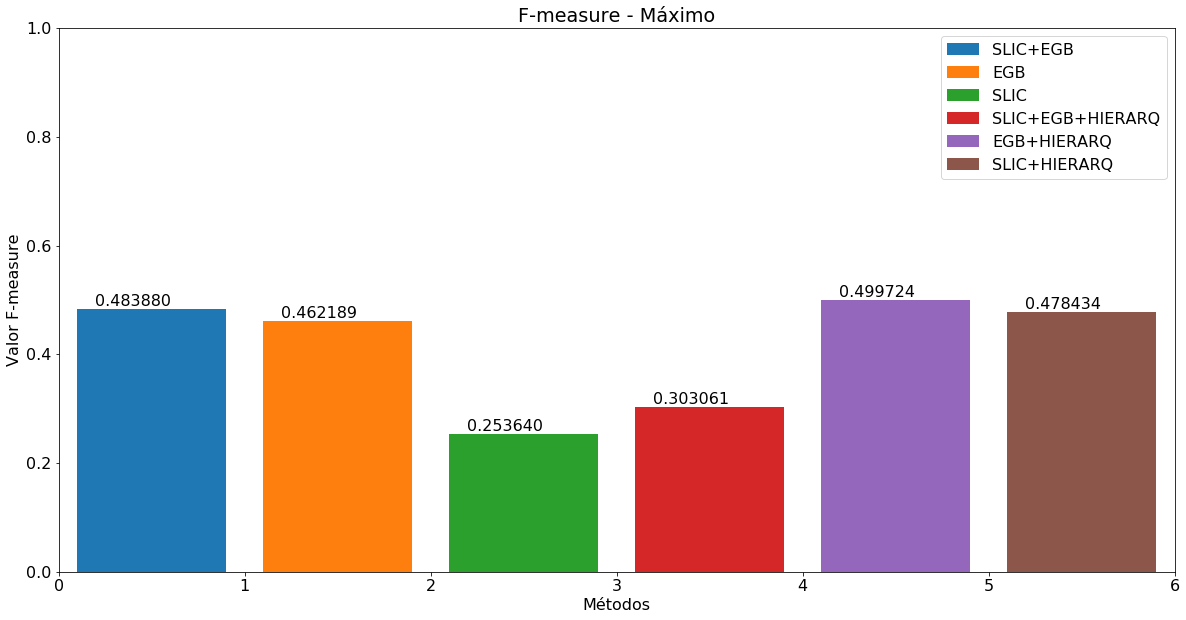
\includegraphics[width=0.5\linewidth]{fmeasure_max.png}}
 \caption{Valor médio e máximo de \textit{F-measure} para os algoritmos.}
\end{figure}

\end{comment}

\begin{figure}[ht]
\centering
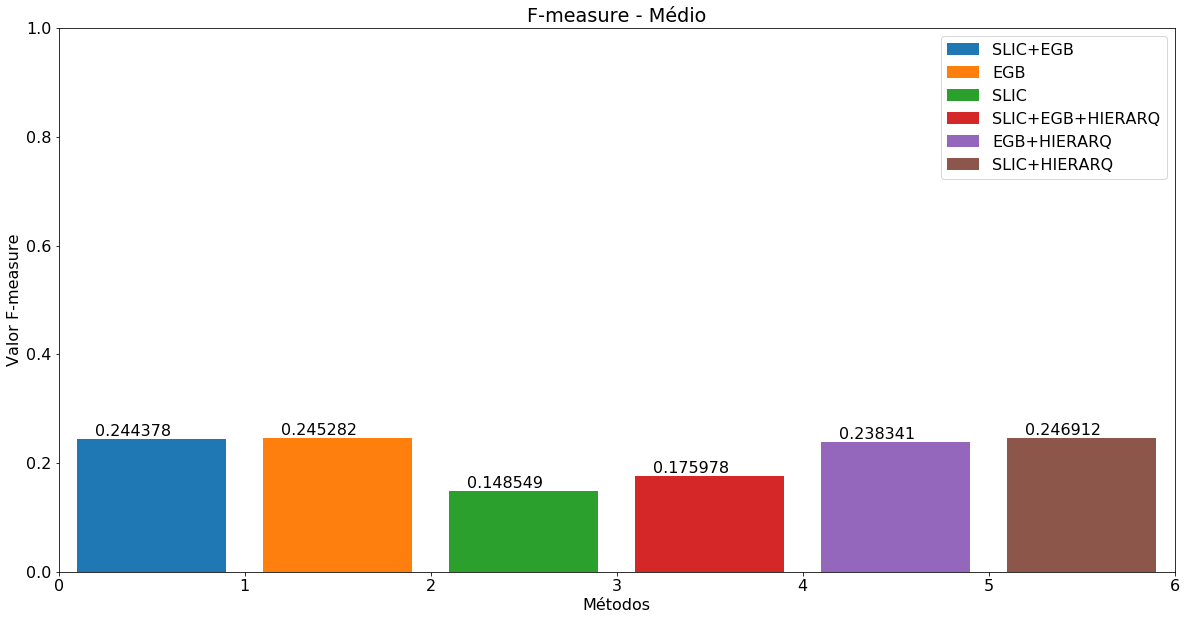
\includegraphics[width=0.9\textwidth]{fmeasure_avg.png}
\caption{Valor médio de \textit{F-measure} para os algoritmos avaliados.}
\label{fig:FMEASURE_AVG}
\end{figure}

Conforme observamos na Figura \ref{fig:FMEASURE_AVG}, o valor médio do algoritmo SEGB teve valores próximois aos obtidos pelo algoritmo EGB. O algoritmo EGB teve valor superior ao algoritmo SLIC, em todos os casos.

Os algoritmos hierárquicos, conforme Figura \ref{fig:FMEASURE_AVG}, resultaram em valores superiores aos algoritmos sem hierarquização. O resultado observado é superior àqueles sem hierarquização. Esse resultado é previsível devido a possibilidade de melhor adequação a base de dados.

Outra análise possível para os algoritmos são os valores máximos de \textit{F-measure}. Esses valores estão ilustrados na Figura \ref{fig:FMEASURE_MAX}. A Figura mostra mais uma vez que as melhores hierarquias obtiveram resultados superiores às versões sem hierarquização. Por fim, vemos que o resultado máximo do algoritmo EGB é superior ao algoritmo SEGB, diferindo do valor médio das amostras.

\begin{figure}[ht]
\centering
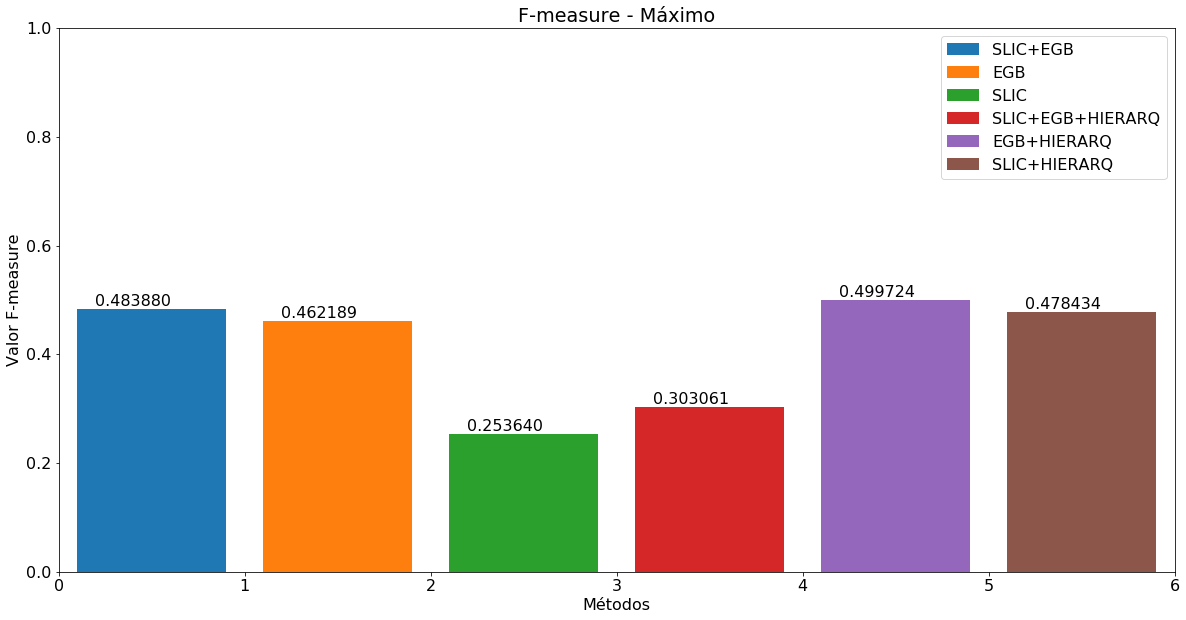
\includegraphics[width=0.9\textwidth]{fmeasure_max.png}
\caption{Valor máximo de \textit{F-measure} para os algoritmos avaliados.}
\label{fig:FMEASURE_MAX}
\end{figure}

%%%%%%%%%%%%%%%%%%%%%%%%%%%%%%%%%%%%%%%%%%%%%%%%%%%%%%%
%%%%%%%%%%%%%%%%%%%%%%%%%%%%%%%%%%%%%%%%%%%%%%%%%%%%%%%

%%%%%%%%%%%%%%%%%%%%%%%%%%%%%%%%%%%%%%%%%%%%%%%%%%%%%%%
%%%%%%%%%%%%%%%%%%%%%%%%%%%%%%%%%%%%%%%%%%%%%%%%%%%%%%%
%%%%%%%%%%%%%%%%%%%%%%%%%%%%%%%%%%%%%%%%%%%%%%%%%%%%%%%

\section{Conclusão} \label{sec:conclusao}

Os algoritmos de geração de superpixels avaliados nesse trabalho tiveram resultados baixos para tarefas de segmentação e detecção de contornos, mesmo quando combinados. As versões hierárquicas dos algoritmos apresentaram resultados superiores àqueles obtidos sem hieraquias.

O algoritmo SLIC, apesar das vantagens de produzir superpixels de tamanhos regulares, apresentou a menor eficiência para segmentação de imagens, em relação aos demais algoritmos estudados. A combinação dos algoritmos SEGB para detecção de contornos não apresentou resultado   superior ao algoritmo EGB. Além disso, o custo computacional para execução dos dois algoritmos em sequência, bem como os custos para recoloração da imagens mostraram-se injustificáveis frente aos ganhos obtidos.

A utilização de hierarquias após a aplicação dos métodos de geração de \textit{superpixels} aumentou consideravelmente os resultados de alguns métodos. Apesar da utilização não resultar em alto grau de desempenho na detecção de bordas e segmentação, justifica-se a utilização das versões hierárquias em relação às versões originais dos algoritmos quando houver necessidade ampliação e redução de contornos, para efeito de agrupamento de informações. Os parâmetros descritos nesse trabalho podem ser utilizados como passo inicial para refinamento dos parâmetros em trabalhos futuros.

Os métodos hierarquicos apresentados no trabalho também permitem a utilização em diferentes cenários, principalmente para redução e agrupamento de informação relevante em imagens, atendendo aos preceitos de análise multiescala.

Como trabalho futuro sugere-se a utilização dos algoritmos mostrados nesse trabalho como passo de pré processamento de outras técnicas de segmentação, como redes neurais convolucionais. Esses passos de segmentação iniciais podem permitir treinamento mais rápido e menor quantidade de informação a ser processadas, além de identificação mais rápida de bordas e contornos.

%%%%%%%%%%%%%%%%%%%%%%%%%%%%%%%%%%%%%%%%%%%%%%%%%%%%%%%
%%%%%%%%%%%%%%%%%%%%%%%%%%%%%%%%%%%%%%%%%%%%%%%%%%%%%%%
%%%%%%%%%%%%%%%%%%%%%%%%%%%%%%%%%%%%%%%%%%%%%%%%%%%%%%%

\bibliographystyle{sbc}
\bibliography{sbc-template}

\end{document}
